% Internal companion draft; no author information is added to this template.
\documentclass[9pt]{osa-supplemental-document}
\setboolean{shortarticle}{false}
\usepackage{amsmath,amsthm,booktabs}
% Keep equation callouts consistent with the main article.
\renewcommand{\eqref}[1]{\textup{(\ref{#1})}}
\newtheorem{proposition}{Proposition}
\renewcommand{\theproposition}{S\arabic{proposition}}
\title{Spectral regularity increases the absolute benefit of response tolerance in reference-matched reflectance design: supplemental document}
\author{}
\begin{abstract}
This document gives the continuous-function support bounds, mixture certificates, tolerance-interval proof, and response-cost calculation supporting the main article. It also proves the smooth-spectrum and input-continuity statements and derives the separate direction and norm comparisons. The accompanying exact fixture contains the rational spectra, response functions, and multipliers needed to verify the numerical inequalities without optimization.
\end{abstract}
\setboolean{displaycopyright}{false}
\begin{document}
\maketitle
\par\medskip
\noindent\textit{Internal companion draft for author revision.}

\section{Input functions and exact representation}
The response interval is $I=[380,780]$ nm, with nodes $\lambda_i=380+i$ for $i=0,\ldots,400$. The CIE 1931 $2^\circ$ observer and the D65, A, and FL11 illuminants are specified by the datasets in Table~\ref{tab:sources}. The FL11 column is selected from the fluorescent-illuminant dataset. Decimal tabulated values are read as exact rational numbers. Each observer and illuminant component is interpolated linearly between nodes.

\begin{table}[htbp]
\centering\small
\caption{Source datasets. The selected interval and interpolation convention, followed by continuous white-Y normalization, define the mathematical model.}
\label{tab:sources}
\begin{tabular}{lll}
\toprule
Input & Year & Dataset DOI\\
\midrule
CIE 1931 observer & 2019 & 10.25039/CIE.DS.xvudnb9b\\
D65 & 2019 & 10.25039/CIE.DS.hjfjmt59\\
A, 1 nm & 2018 & 10.25039/CIE.DS.8jsxjrsn\\
Fluorescent illuminants, 1 nm & 2018 & 10.25039/CIE.DS.54hy6srn\\
\bottomrule
\end{tabular}
\end{table}

If $E_j$ is an illuminant and $\overline x,\overline y,\overline z$ are the matching functions, then
\begin{equation}
 f_j(\lambda)=\frac{100E_j(\lambda)}{\int_I E_j\overline y}
 \begin{pmatrix}\overline x(\lambda)\\\overline y(\lambda)\\\overline z(\lambda)\end{pmatrix}.
 \label{eq:kernel}
\end{equation}
Every component of $f_j$ is quadratic on each bin. The normalization is evaluated by exact integration of the product; it is not a rectangle sum over nodes. Positive scalar factors already present in a stored illuminant cancel in Eq.~\eqref{eq:kernel}.

Let $N_i$ denote the standard continuous piecewise-linear hat functions. The exact nine-moment matrix is
\begin{equation}
 T_{(j,k),i}=\int_I f_{j,k}N_i,
 \quad j=0,1,2,\quad k=X,Y,Z.
\end{equation}
For a nodal spectrum $z=\sum_i z_iN_i$, its nine responses are $Tz$. The fixture contains a nonsingular nine-column minor and its rational inverse. Multiplication by the saved inverse is checked exactly. This verifies full row rank and supports the finite-dimensional corrections used below.

For each lower-bound witness, the verifier checks $|z_i|\leq1/2$ and the exact response equations. In class $\mathcal S$ it also checks $\ell\leq z_{i+1}-z_i\leq u$ on every 1 nm bin. These endpoint inequalities imply passivity and the derivative bounds on the complete piecewise-linear function. All numerical bounds concern the interpolated model of Eq.~\eqref{eq:kernel}.

\section{Mixtures and normalization}
For $w_j\geq0$, let $c_w=\sum_jw_jc_j$, $h_w=\sum_jw_jh_j$, and $e_w=\sum_jw_je_j$. If $K$ is attained by a named illumination and
\begin{equation}
 K^2c_i^{\mathsf T}c_j-h_i^{\mathsf T}h_j\geq0\quad\text{for every }i,j,
\end{equation}
then $\|h_w\|_2^2\leq K^2\|c_w\|_2^2$. Thus the same $K$ is the maximum over the full cone. Similarly, the sufficient conditions
\begin{equation}
 \rho^2\beta^2K^2c_i^{\mathsf T}c_j-e_i^{\mathsf T}e_j\geq0
 \quad\text{for every }i,j
 \label{eq:errorgram}
\end{equation}
prove the error condition for every mixture. These are sufficient copositivity certificates obtained through entrywise nonnegativity, not necessary conditions for arbitrary error vectors.

The scalar $K^2$, squared norms, and Gram entries are rational. All four X-direction witnesses used in the capacity comparison pass the appropriate mixture checks. The Z-direction comparison uses an exact lower witness, so its zero errors extend to mixtures directly. No approximate Z witness is needed for that comparison.

Named-lamp upper bounds are valid for the all-mixture problem because the latter includes the named conditions. Combined with mixture-feasible lower witnesses, this gives the same reported enclosures for the two domains. It does not identify their unknown exact capacities with one another.

\section{Support certificates on continuous function classes}
\subsection{Multiplier inequality and the unrestricted class}
Write $h_j=Hc_j$ and $e_j=A_jz-\beta h_j$. For fixed multiplier vectors,
\begin{equation}
 g=\sum_j\mu_j^{\mathsf T}f_j,\qquad P=\sum_j\mu_j^{\mathsf T}h_j.
\end{equation}
Then $\int_Igz=\beta P+\sum_j\mu_j^{\mathsf T}e_j$. The reference term is zero, while Cauchy--Schwarz bounds each remaining term below by $-\rho\beta K\|c_j\|_2\|\mu_j\|_2$. For an outward upper bound $W$ on their summed coefficients,
\begin{equation}
 \beta(P-\rho W)\leq\int_Igz.
 \label{eq:dualsupport}
\end{equation}
Over $\mathcal U$, the support is exactly $\tfrac12\int_I|g|$. Division by a positive $P-\rho W$ gives a rigorous upper capacity bound, irrespective of whether the multipliers are optimal.

For a polynomial $p(t)=\sum_{i=0}^n b_iB_i^n(t)$ in Bernstein form on $[0,1]$,
\begin{equation}
 \frac{|\sum_i b_i|}{n+1}\leq\int_0^1|p(t)|\,dt
 \leq\frac{\sum_i|b_i|}{n+1}.
 \label{eq:bernstein}
\end{equation}
The right inequality uses nonnegativity of the basis; the left is the absolute value of the integral. Rational subdivision tightens these enclosures. A coordinate change to a physical bin of width $h$ multiplies the integral by $h$. The verifier retains that factor on every subinterval, including the half-bin intervals of the cubic certificate.

\subsection{Nodal support and the continuous correction}
For nodal values $v=(v_0,\ldots,v_{400})$, let $(Dv)_i=v_{i+1}-v_i$. Let $a_i=\int_IgN_i$. For any multiplier vector $\eta$ on the differences, put $q=a-D^{\mathsf T}\eta$. Then
\begin{equation}
 a^{\mathsf T}v=\eta^{\mathsf T}Dv+q^{\mathsf T}v
 \leq\sum_i\max(\ell\eta_i,u\eta_i)+\frac12\|q\|_1.
 \label{eq:nodalsupport}
\end{equation}
This support inequality uses only the passive and slope restrictions. In particular, it imposes no response-equality condition on the interpolant to which it is applied.

For $z\in\mathcal S$, its endpoint interpolant $Lz$ satisfies those restrictions. On one unit bin write $g(t)=a+bt+ct^2$ and $z(t)=z(0)+\int_0^t z'(s)ds$. Subtracting $(1-t)z(0)+tz(1)$ and exchanging integrals gives
\begin{align}
 \int_0^1g(z-Lz)&=\int_0^1 K_P(s)z'(s)ds,\\
 K_P(s)&=\int_s^1g(t)dt-\int_0^1tg(t)dt\\
 &=a/2+b/6+c/12-as-bs^2/2-cs^3/3.
\end{align}
The kernel has zero integral. Subtract $(\ell+u)/2$ from $z'$ inside the last integral to obtain
\begin{equation}
 \left|\int_0^1g(z-Lz)\right|\leq\frac{u-\ell}{2}\int_0^1|K_P|.
 \label{eq:peanobound}
\end{equation}
Summing Eq.~\eqref{eq:peanobound} over all bins and adding Eq.~\eqref{eq:nodalsupport} bounds $\int_Igz$ for every absolutely continuous spectrum in the envelope. The exact-response capacity bound divides by $P>0$. Numerically, the finite support contributes approximately 0.2101706137820 to the amplitude upper, and the continuous correction contributes approximately 0.00702177349656. Their certified sum is the upper $B_0$ used in the main theorem.

\subsection{A continuous cubic support bound}
Let $\phi$ be continuous and piecewise cubic, with $\phi(380)=\phi(780)=0$. For every $z\in\mathcal S$,
\begin{align}
 \int_Igz&=-\int_I\phi z'-\int_I(\phi'-g)z\\
 &\leq\frac{u-\ell}{2}\int_I|\phi|
 -\frac{u+\ell}{2}\int_I\phi+\frac12\int_I|\phi'-g|.
 \label{eq:cubicsupport}
\end{align}
The first term follows by maximizing $-\phi z'$ pointwise over $z'\in[\ell,u]$; the second uses the passive box. The fixture supplies $\phi$ and $\mu$. Exact continuity and endpoint checks validate the integration by parts. Polynomial differentiation, residual construction, and Bernstein integration then give the full-S tolerant upper bound. This upper need not equal the optimum of a nodal optimization problem.

\section{Absolute bonus and tolerance interval}
\subsection{Capacity arithmetic}
Use the four capacity intervals in the main article and denote lower and upper endpoints by superscripts $-$ and $+$. Then, for example,
\begin{align}
 \Delta_{\mathcal S}(r)&\geq b_{\mathcal S}^-(r)-b_{\mathcal S}^+(0)/(1-r),\\
 \Delta_{\mathcal U}(r)&\leq b_{\mathcal U}^+(r)-b_{\mathcal U}^-(0)/(1-r).
\end{align}
At $r=0.10$, exact cross-multiplication proves that the first lower bound exceeds 1.50 times the second upper bound. The reverse endpoint combinations give the remaining interval endpoints and establish a positive unrestricted bonus. The raw increments have enclosures
\begin{align}
 b_{\mathcal S}(r)-b_{\mathcal S}(0)&\in(0.1855354858,0.2762275169),\\
 b_{\mathcal U}(r)-b_{\mathcal U}(0)&\in(0.1292643479,0.1499960386).
\end{align}
The lower difference is greater than 0.0355394472. The exact penalty obeys $d(0)<0.1733445365$, giving the main article's conservative reduction fraction of 0.2160. The stricter rational calculation gives a lower fraction exceeding 0.21600115.

\subsection{Feasible interpolation below the anchor tolerance}
Let $(z_0,b_0)$ be the exact S witness and $(z_1,b_1)$ the witness at $r=0.10$. For $0\leq t\leq1$, define
\begin{equation}
 z_t=(1-t)z_0+tz_1,\qquad\beta_t=(1-t)b_0+tb_1.
\end{equation}
Convexity preserves the spectral constraints and reference equality. The error is $t$ times that of $z_1$, so a sufficient tolerance is $x=trb_1/\beta_t$. Solving for $t$ yields
\begin{equation}
 \beta_t=\frac{b_0}{1-kx},\qquad
 k=\frac{b_1-b_0}{rb_1},\qquad0\leq x\leq r.
 \label{eq:blendexact}
\end{equation}
The same calculation is valid for the full mixture domain because both endpoint witnesses satisfy all of its constraints.

For $r\leq x<1$, keep $z_1$ and set $\beta=(1-r)b_1/(1-x)$. Then $\beta\geq b_1$, and
\begin{equation}
 \|A_wz_1-\beta h_w\|_2
 \leq[rb_1+(\beta-b_1)]K\|c_w\|_2
 =x\beta K\|c_w\|_2.
\end{equation}
This proves the upper-tolerance lower curve without a new solve.

\begin{table}[htbp]
\centering
\caption{Constants used in the tolerance and norm comparisons. Values shown are decimal summaries; the rational fixture determines the signs in the proof.}
\label{tab:constants}
\begin{tabular}{cll}
\toprule
Symbol & Meaning & Approximate value\\
\midrule
$b_0$ & exact S witness & 0.2101706137814355\\
$b_1$ & tolerant S witness & 0.4027278731222646\\
$B_0$ & exact S upper & 0.21719238727858622\\
$U_0$ & exact U lower & 0.38172598678848113\\
$L$ & unrestricted support upper & 0.051541722172949694\\
$P$ & target pairing for that support & 0.13027912697583505\\
$W$ & outward error coefficient & 0.333455419161111\\
$k$ & blend coefficient & 4.781324367940393\\
\bottomrule
\end{tabular}
\end{table}

\subsection{Whole-interval sign proof}
Set $D_0=U_0-B_0>0$. Below $r$, a lower bound for the bonus difference is
\begin{equation}
 F(x)=\frac{b_0}{1-kx}-\frac{L}{P-Wx}+\frac{D_0}{1-x}.
\end{equation}
Multiplication by $(1-kx)(P-Wx)(1-x)>0$ gives
\begin{multline}
 q(x)=b_0(P-Wx)(1-x)-L(1-kx)(1-x)\\
 +D_0(1-kx)(P-Wx).
\end{multline}
Its coefficients are checked exactly: the constant is negative and the linear and quadratic coefficients are positive. Hence $q$ is strictly increasing for $x\geq0$. The rational sign $q(0.056736)>0$ proves positivity throughout $[0.056736,r]$.

Above $r$, the lower difference is
\begin{equation}
 \frac{(1-r)b_1+D_0}{1-x}-\frac{L}{P-Wx}.
\end{equation}
Its numerator after multiplication by the positive denominators is affine and decreasing. It remains positive at $x=0.137809$, proving the second half of the interval. The same rational checks verify denominator positivity throughout. The plot of these functions illustrates this argument but is not used to establish it.

\section{Universal actual responses and the signed A-Y cost}
\subsection{Ball and half-space relaxation}
For the exact S support let $L_{\mathcal S}=P_{\mathcal S}B_0$. At amplitude $\beta$, every feasible design satisfies
\begin{equation}
 \mu_1^{\mathsf T}e_1+\mu_2^{\mathsf T}e_2\leq L_{\mathcal S}-\beta P_{\mathcal S}.
\end{equation}
For $j\in\{1,2\}$ and the other index $o=3-j$, put
\begin{equation}
 C_j=P_{\mathcal S}-\rho K\|c_o\|_2\|\mu_o\|_2,
 \quad B_j=L_{\mathcal S}-\beta C_j,
 \quad T_j=\beta\rho K\|c_j\|_2.
\end{equation}
The error lies in $\{e:\|e\|_2\leq T_j,\ \mu_j^{\mathsf T}e\leq B_j\}$. This set is a relaxation of the spectral problem. Any upper bound on a coordinate over it applies to every feasible spectrum.

For a unit vector $a$ and nonzero $\mu$, let $p=a^{\mathsf T}\mu$, $s^2=\|\mu\|_2^2$. If $pT\leq B$, the unconstrained ball maximizer $Ta$ is feasible. Otherwise, at a nonempty cap with $-sT\leq B<sT$, the optimum lies in the plane $\mu^{\mathsf T}e=B$. Decompose
\begin{equation}
 e=\frac{B}{s^2}\mu+v,\qquad v\perp\mu,\qquad
 \|v\|_2\leq\sqrt{T^2-B^2/s^2}.
\end{equation}
The projection of $a$ into that plane has norm $\sqrt{1-p^2/s^2}$, giving
\begin{equation}
 \max a^{\mathsf T}e=\frac{pB+\sqrt{s^2-p^2}\sqrt{s^2T^2-B^2}}{s^2}.
\end{equation}
An empty cap excludes feasibility altogether. Every branch choice used at the stated amplitude is checked using outward rational intervals.

\subsection{Numerical consequences and extension to larger amplitudes}
At $\beta_*=b_1$, the A values are approximately
\begin{equation}
 \mu_1=(0.00545967376,0.04593605206,-0.00767597078)^{\mathsf T},
\end{equation}
with $C_1\simeq0.09250594414$, $B_1\simeq-0.01620148977$, and $T_1\simeq0.59630591471$. Evaluating the cap for $a=e_Y$ and $a=-e_X$ gives the necessary Y deficit and the actual-X lower bound in the main article. Under FL11, the X cap bound reduces to the ordinary error-ball bound, and no positive universal Y deficit follows.

Normalize by amplitude, $v_j=e_j/\beta$. The constraints become
\begin{equation}
 \|v_j\|_2\leq\rho K\|c_j\|_2,\quad
 \mu_j^{\mathsf T}v_j\leq L_{\mathcal S}/\beta-C_j.
\end{equation}
These sets decrease with $\beta$. At $\beta_*$ the bound for the actual X response per unit amplitude is positive, and the A-Y upper per unit amplitude is negative. Multiplying by any larger feasible amplitude preserves and strengthens the absolute inequalities. This proves the all-feasible quantifier above the threshold.

If $e_{1,Y}\geq0$ and $\mu_{1,Y}>0$, the most negative support contribution in the A ball occurs with $e_{1,Y}=0$. Therefore
\begin{equation}
 \beta\leq\frac{L_{\mathcal S}}
 {C_1-\rho K\|c_1\|_2\sqrt{\mu_{1,X}^2+\mu_{1,Z}^2}}
 <0.2679937276830.
\end{equation}
The denominator is certified positive. This bound establishes exclusion of the $\beta_*$ regime when no A-Y loss is allowed, without claiming the bound is an attained fixed-Y optimum.

\section{Smooth-spectrum capacity suprema}
Let $Mz$ collect the nine response moments. The kernels are bounded on $I$ and $M$ has full rank on a finite piecewise-linear span. Choose nine functions with independent moment columns. Smooth compactly supported functions approximate them in $L^1(I)$, so boundedness of the kernels and determinant continuity provide fixed $\psi_i\in C_c^\infty(\operatorname{int}I)$ with invertible moment matrix $V$. Define
\begin{equation}
 Rq=\sum_i\psi_i(V^{-1}q)_i.
\end{equation}
Then $MRq=q$, and there are finite constants $C_0,C_1$ such that $\|Rq\|_\infty\leq C_0\|q\|_\infty$ and $\|(Rq)'\|_\infty\leq C_1\|q\|_\infty$.

\begin{proposition}
For every $z\in\mathcal U$ and $0<\theta<1$, there is a smooth $z_\infty\in\mathcal U$ with $Mz_\infty=\theta Mz$. If $z\in\mathcal S$, $z_\infty$ can be chosen in $\mathcal S$.
\end{proposition}
\begin{proof}
For $\mathcal U$, extend $\theta z$ by zero and convolve with a nonnegative compactly supported smooth approximate identity. The result $g_\varepsilon$ satisfies $|g_\varepsilon|\leq\theta/2$ and converges in $L^1(I)$ to $\theta z$. Hence $q_\varepsilon=\theta Mz-Mg_\varepsilon\to0$. The function $g_\varepsilon+Rq_\varepsilon$ has exactly the desired moments and stays inside the passive box for sufficiently small $\varepsilon$.

For $\mathcal S$, extend $z$ constantly beyond the endpoints. Its derivative remains in $[\ell,u]$, since $0\in[\ell,u]$. Mollification of $\theta z$ yields $\theta\ell\leq g_\varepsilon'\leq\theta u$, preserves the contracted passive box, and converges uniformly. Choose $\varepsilon$ small enough that
\begin{equation}
 C_0\|q_\varepsilon\|_\infty<(1-\theta)/2,\qquad
 C_1\|q_\varepsilon\|_\infty<(1-\theta)\min(-\ell,u).
\end{equation}
The correction then fits both spectral margins and restores all nine moments exactly.
\end{proof}

The response constraints are positively homogeneous in $(Mz,\beta)$. Thus $(z_\infty,\theta\beta)$ is feasible whenever $(z,\beta)$ is feasible. All mixture responses follow from the exact generator moments. Taking $\theta\uparrow1$, and using inclusion for the reverse inequality, proves equality of the original and smooth-subclass capacity suprema. The construction does not impose a common second-derivative bound or prove smooth attainment at an endpoint amplitude.

\section{Continuity with respect to input functions}
Let $p$ index response kernels converging componentwise in $L^1(I)$ to those at $p_0$, with continuous target vectors $h_{p,j}$ and $h_{p,0}=0$. The derivative interval is fixed with $\ell<0<u$. Assume full moment rank at $p_0$, uniformly positive $\|c_p(w)\|_2$ on the compact mixture simplex, and a nonzero target. Define $K_p$ by maximization over that simplex or over the named lamps. Uniform convergence of numerator and denominator gives continuity of $K_p>0$.

The preceding smooth basis has moment matrices $V_p\to V_{p_0}$. Thus $R_pq=\sum_i\psi_i(V_p^{-1}q)_i$ is a locally uniformly bounded right inverse in both the function and derivative norms. Small positive multiples of $R_ph_p$ are exact feasible designs, ensuring positive exact capacity nearby.

For upper semicontinuity, the triangle inequality at an illumination attaining $K_p$ provides a uniform upper bound on feasible amplitudes. In $\mathcal U$, weak-star compactness gives a subsequential limit; $L^1$ kernel convergence and bounded spectra imply convergence of moments. In $\mathcal S$, boundedness and a common Lipschitz constant give uniform subsequential convergence. The inequalities $\ell(y-x)\leq z(y)-z(x)\leq u(y-x)$ pass to that limit. In either class the reference and every fixed-mixture response constraint pass to the limit, proving
\begin{equation}
 \limsup_{p\to p_0}b_{\mathcal C,p}(\rho)\leq b_{\mathcal C,p_0}(\rho).
\end{equation}

At $\rho=0$, contract an exact feasible design by $\theta<1$ and correct its moments with
\begin{equation}
 q_p=\theta\beta h_p-M_p(\theta z),\qquad z_p=\theta z+R_pq_p.
\end{equation}
The correction tends to zero and fits the strict spectral margins. This yields lower semicontinuity at exact tolerance.

At $0<\rho<1$, first blend a feasible pair $(z,\beta)$ with a positive exact pair $(z_e,\beta_e)$ in the same class:
\begin{equation}
 \bar z=(1-\delta)z+\delta z_e,\qquad
 \bar\beta=(1-\delta)\beta+\delta\beta_e.
\end{equation}
The error becomes $(1-\delta)e(w)$, and its cone slack is at least $\rho\delta\beta_eK_{p_0}\|c_{p_0}(w)\|_2$, uniformly positive on the simplex. Contract by $\theta<1$ for spectral slack, then prescribe the generator moments
\begin{equation}
 d_p=\theta[\bar\beta h_p+(1-\delta)e],\quad
 q_p=d_p-M_p(\theta\bar z),\quad
 z_p=\theta\bar z+R_pq_p.
\end{equation}
The corrected spectrum has reference error zero and mixture errors $\theta(1-\delta)e(w)$. Continuity preserves the strict cone slack, and the small correction fits the spectral margins. Letting $\theta\uparrow1$ and $\delta\downarrow0$ proves lower semicontinuity. Capacities, and hence the bonus difference at fixed $\rho$, are continuous. The strict central inequality persists in some neighborhood of the frozen inputs. This argument gives no numerical radius for measurement or interpolation uncertainty.

\section{Separate direction and norm comparisons}
\subsection{The X and Z directions in common units}
For $d=X,Z$, define $\Phi_d=K_d[b_{\mathcal S,d}(0.10)-b_{\mathcal S,d}(0)/0.9]$. Target inflation gives $\Phi_d\geq0$. The X lower is the central S bonus lower multiplied by an outward lower enclosure of $K_X$. The Z upper is the full-AC tolerant upper, obtained by the nodal support and Peano correction, minus an exact Z witness amplitude divided by 0.9, then multiplied by an outward upper enclosure of $K_Z$. Let these two positive certificate endpoints be $A$ and $B$. They satisfy
\begin{equation}
 A>0.0156453680148,\qquad B<0.0003455399445,\qquad A>45.278B>0.
\end{equation}
Consequently $\Phi_X>45.278\Phi_Z$. This statement remains valid when the unknown actual Z bonus is zero; no ratio with a zero actual bonus is taken.

\begin{figure}[htbp]
\centering
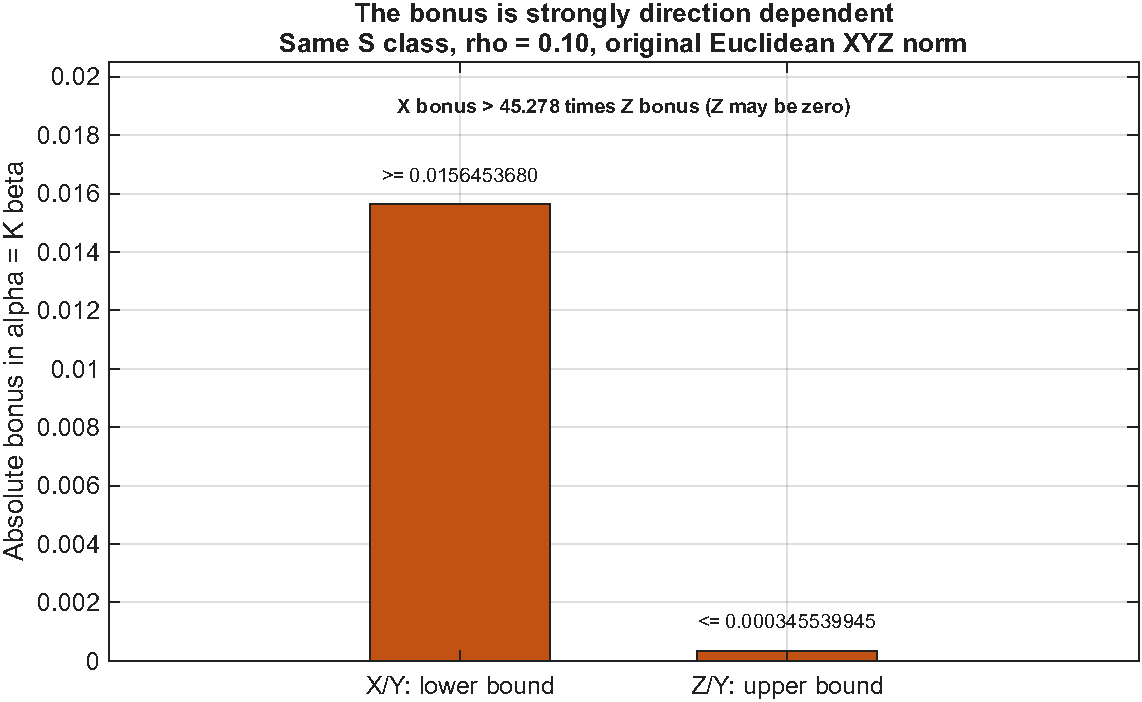
\includegraphics[width=\linewidth]{figures/04-common-alpha-direction.pdf}
\caption{Euclidean direction comparison in common $\alpha=K\beta$ units. The X lower bonus exceeds 45.278 times the Z upper bonus. This comparison concerns two fixed transformations and is separate from the norm perturbation result.}
\end{figure}

\subsection{A sufficient linear-norm radius}
Let $D$ be an invertible real $3\times3$ matrix used on error, target, and incident response. With $\kappa=\operatorname{cond}_2(D)$, singular-value bounds imply $K_I/\kappa\leq K_D\leq\kappa K_I$. The normalized error criterion $J_D$ therefore satisfies
\begin{equation}
 \kappa^{-2}J_I\leq J_D\leq\kappa^2J_I.
\end{equation}
For $t\geq\kappa^2$ this yields
\begin{equation}
 b_{\mathcal C,I}(r/t)\leq b_{\mathcal C,D}(r)\leq b_{\mathcal C,I}(rt),
 \qquad b_{\mathcal C,D}(0)=b_{\mathcal C,I}(0).
\end{equation}
The exact baseline is unchanged by an invertible coordinate map. The inflation subtraction remains $b_{\mathcal C}(0)/(1-r)$ in both comparisons. Using Table~\ref{tab:constants},
\begin{align}
 \Delta_{\mathcal S,D}(r)&\geq b_0/(1-kr/t)-B_0/(1-r),\\
 \Delta_{\mathcal U,D}(r)&\leq L/(P-rWt)-U_0/(1-r).
\end{align}
Multiplying the difference by $(1-r)(t-kr)(P-rWt)>0$ gives
\begin{multline}
 q_D(t)=b_0t(P-rWt)(1-r)-L(t-kr)(1-r)\\
 +D_0(t-kr)(P-rWt).
\end{multline}
The quadratic coefficient is negative, $q_D'(1)<0$, and $q_D(1)>0$. Exact rational evaluation also gives $q_D(1.052918^2)>0$, with all denominators positive over that interval. Since the derivative decreases, the polynomial is positive throughout $1\leq t\leq1.052918^2$. This proves the sufficient condition-number bound in the main article. At $\kappa\leq1.02$, the lower S and upper U bounds are approximately 0.1475673909 and 0.1150759345. No assumption is made that the lamp attaining $K_D$ remains unchanged.

\section{Reproduction and verification status}
The accompanying directory \texttt{reproducibility/} is a self-contained subset of the research files. It contains the exact fixture, the verified display export, a standard-library Python checker, and a MATLAB presentation function. From that directory, run
\begin{verbatim}
python -B tools/verify_paper_results.py
\end{verbatim}
The default is read-only. It reconstructs the integrated model, checks rank, verifies the five selected X/Z witnesses, evaluates full-class supports, and checks the absolute, interval, cost, and scope inequalities. It needs no optimizer, network access, machine configuration, or historical project imports. Assertions must remain enabled; the script rejects Python optimization mode.

For an explicitly writable export followed by presentation checks, use
{\footnotesize
\begin{verbatim}
python -B tools/verify_paper_results.py --emit results/research/R135-paper-verified.json
\end{verbatim}
}
and, from MATLAB in the same directory,
\begin{verbatim}
run_paper_results('verify')
run_paper_results('render')
\end{verbatim}
Rendering uses the verified scalar export and checks its fixture hash. It creates deterministic plots and tables without optimization. The saved rendering was produced with MATLAB R2025b; the exact checker was verified with Python 3.12.14. The display values use floating-point conversion, while the certificates use rational arithmetic and outward radical enclosures.

The original tolerant S solver's non-success flag is retained in the fixture. Its lower bound is justified by the subsequently repaired exact feasible spectrum, not by a claim of successful optimizer termination. The support endpoints are rigorous bounds, not necessarily attained extrema. The smooth-spectrum and continuity propositions are analytical proofs; the arithmetic checker is not a proof-assistant formalization of them.

The frozen fixture's SHA-256 digest is
\begin{quote}\ttfamily\small
89c4a74ed3c54a05df04d8176cc3e8105\\
dcb84040799718314ab5246bcfd58d7.
\end{quote}
The line break and final punctuation are not part of the digest. The package preserves input and source hashes, source dataset attribution, and the history of the numerical certificates. Author details and publication declarations are maintained separately from these technical files.
\end{document}
